\chapter{Directory Structure}

We briefly describe the directory structure of \Dumux in terms 
of subdirectories, source files, and tests. For more details, 
the Doxygen documentation should be considered. 
\Dumux comes in form of a DUNE module \texttt{dumux}. 
It has a similar structure as other DUNE modules like \texttt{dune-grid}. 
The following subdirectories are within the module's root directory, 
from now on assumed to be \texttt{/}: 
\begin{itemize} 
\item \texttt{CMake}: the configuration options 
for building \Dumux using CMake. See the file \texttt{INSTALL.cmake} in 
the root directory of \texttt{dumux} for details. Of course, 
it is also possible to use the DUNE buildsystem just like for the other 
DUNE modules.
\item \texttt{doc}: contains the Doxygen documentation in \texttt{doxygen}, 
this handbook in \texttt{handbook}, and the \Dumux logo in various formats in 
\texttt{logo}. The html documentation produced by Doxygen can be accessed as usual, 
namely, by opening \texttt{doc/doxygen/html/index.html} with a web browser. 
\item \texttt{dumux}: the \Dumux source files. See Section \ref{sec:dumux} for details. 
\item \texttt{test}: tests for each numerical model and the property system. 
See Section \ref{sec:test} for details. 
\item \texttt{tutorial}: contains the tutorials described in Chapter \ref{chp:tutorial}. 
\end{itemize}



\section{The directory \texttt{dumux}}\label{sec:dumux}

The directory \texttt{dumux} contains the \Dumux source files. It consists of the following subdirectories (see Figure \ref{fig:dumux-structure}): 

\begin{itemize} 

\item \texttt{boxmodels}:
the general fully implicit box method is contained in the subdirectory 
\texttt{common}, while each of the other subdirectories contains 
a derived specific numerical model. The subdirectory \texttt{common} also contains the file \texttt{boxfvelementgeometry.hh} employed by the box method to extract the dual mesh geometry information out of the primal one. The files \texttt{pdelabboxassembler.hh} and \texttt{pdelabboxlocaloperator.hh} allow the use of the DUNE module \texttt{dune-pdelab}. 

\item \texttt{common}:
general stuff like the property system and the time management for the 
fully coupled as well as the decoupled models, the interface for the Pardiso direct solver library \cite{Pardiso}, and the \texttt{start.hh} file that includes the common routine for starting a model called in the main function. 

\item \texttt{decoupled}:
 numerical models to solve the pressure equation as part of the fractional flow formulation. The specific models are contained 
 in corresponding subdirectories. In each model folder are subdirectories for the implicit pressure equation sorted by the employed discretization method, and for the explicit transport equation. The general decoupled formulation for the implicit pressure explicit transport formulation can be found in the subdirectory \texttt{common}.

% \item \texttt{fractionalflow}:
% the (non-compositional) fractional flow model, which utilizes the IMPES method 
% contained in the subdirectory \texttt{impes}.

% \item \texttt{functions}:
% the Crouzeix--Raviart function implemented in the style of \texttt{dune-disc}'s P1 function. 

% \item \texttt{fvgeometry}:
% employed by the box method to extract the dual mesh geometry information out of the 
% primal one. 

\item \texttt{io}: additional in-/output possibilities like restart files 
and a VTKWriter extension. 

\item \texttt{material}: everything related to material parameters and 
constitutive equations. The properties of a pure chemical substance (e.g. water) or pseudo substance (e.g. air) can be found in the subdirectory \texttt{components} with the base class \texttt{components/component.hh}. The fluidsytem in the folder \texttt{fluidsystems} collects the information from the respective component and binary coefficients files, and contains the fluid characteristics of phases (e.g. viscosity, density, enthalpy, diffusion coefficients) for compositional or non-compositional multi-phase flow. 

The base class for all spatially dependend variables -- like permeability and porosity  -- 
can be found in \texttt{spatialparameters}. The base class in \texttt{boxspatialparameters.hh} 
also provides spatial averaging routines. All other spatial properties are specified in the specific
 files of the respective models. Furthermore, the constitutive relations -- e.g. $p_c(S_w) $ -- are in \texttt{fluidmatrixinteractions}, 
while the necessary binary coefficients like the Henry coefficient or binary diffusion coefficients are definded in
 \texttt{binarycoefficients}.


\item \texttt{nonlinear}: Newton's method.


% \item \texttt{operators}: based on \texttt{dune-disc}, assembly operators for Crouzeix--Raviart 
% elements and mimetic finite differences. 
% 
% 
% \item \texttt{pardiso}: interface to the Pardiso direct solver library, \cite{Pardiso}. 
% 
% 
% \item \texttt{shapefunctions}:  Crouzeix--Raviart element shape functions. 
% 
% 
% \item \texttt{timedisc}: time discretization for the decoupled models. 
% 
% 
% \item \texttt{transport}: numerical models to solve the pressure equation 
% as part of the fractional flow formulation analogous to the \texttt{diffusion} 
% directory. Moreover, the compositional decoupled models are included here. 


\end{itemize}



\section{The directory \texttt{test}}\label{sec:test}


The directory \texttt{test} contains a test for each numerical model and for 
the property system. The tests for the property system and the pardiso solver can be found in \texttt{common}. 
The subfolder \texttt{boxmodels} contains tests for the fully 
coupled models (\texttt{1p},  \texttt{1p2c},  \texttt{2p},  \texttt{2p2c},  
\texttt{2p2cni},  \texttt{2pni},  and \texttt{richards}), while the subdirectory \texttt{decoupled} corresponds to the decoupled models. 
Each subdirectory contains one or more program files \texttt{test\_*.cc}, where \texttt{*} usually is the 
name of the folder. Moreover, the problem definitions can be found 
in the \texttt{*problem.hh} files and the definition of the spatially dependend parameters in \texttt{*spatialparameters.hh}. Simply executing the tests should either run the 
full test or give a list of required command line arguments. After test execution, 
VTK output files should have been generated. 
For more detailed descriptions of the tests, the problem definitions and their corresponding 
Doxygen documentation should be considered. 

\begin{landscape}
\begin{figure}[hbt]
  \centering 
  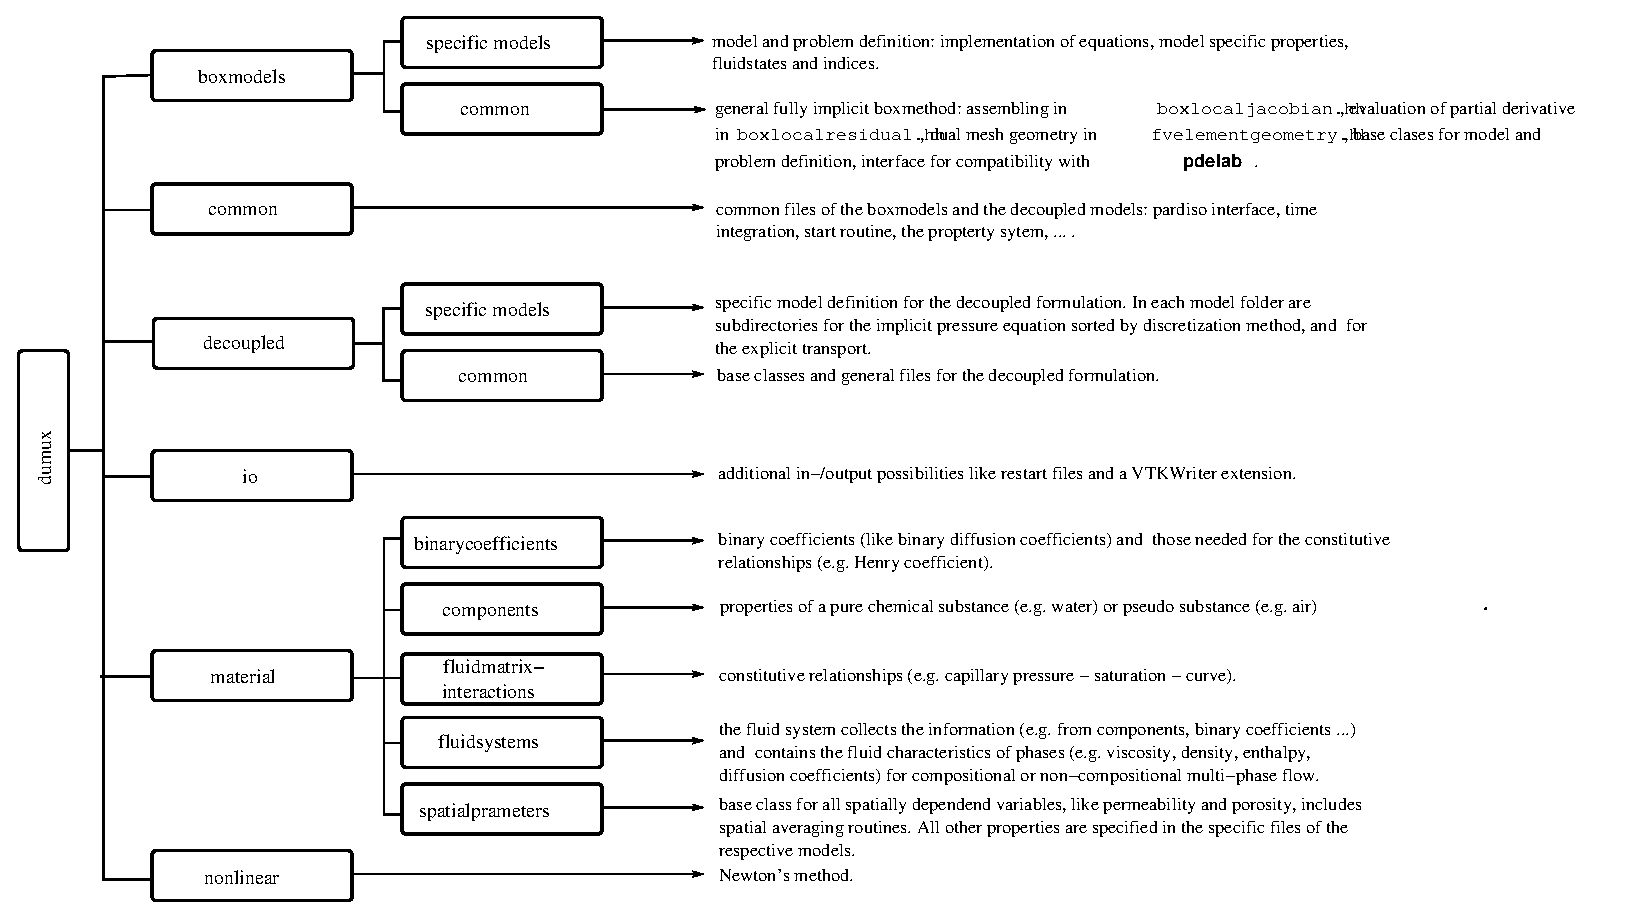
\includegraphics[width=\linewidth, keepaspectratio]{EPS/dumux_strucutre_flowchart_horizontal_explained.eps}
  \caption{
    \label{fig:dumux-structure}
    Structure of the directory \texttt{dumux} containing the \Dumux source files.
  }
\end{figure}
\end{landscape}
